% Capítulo 2 - Marco Teórico 
\chapter{Marco Teórico}
\label{cap:MarcoTeorico}
En este capítulo se describen los conceptos teóricos y el estado del arte necesarios para comprender el desarrollo y las decisiones de arquitectura tomadas para la realización de este Trabajo de Fin de Máster. 

Dada la naturaleza compleja y multimodal del problema abordado (la detección y categorización del sexismo en redes sociales), el marco teórico abarca desde los principios fundamentales del Aprendizaje Automático y Profundo (\textit{Deep Learning}) hasta los enfoques más modernos en Procesamiento del Lenguaje Natural y Visión Artificial. A lo largo de las siguientes secciones, se realiza una revisión crítica de las arquitecturas de estado del arte, prestando especial atención a los modelos basados en Transformers y a los Grandes Modelos de Lenguaje (\textit{LLMs}). Asimismo, se fundamentan de manera teórica las estrategias empleadas para la experimentación, como el aprendizaje por transferencia, la fusión de modelos (\textit{ensembles}) y el novedoso paradigma del aprendizaje con desacuerdo (\textit{LeWiDi}), justificando su idoneidad para modelar la subjetividad y el sesgo en las plataformas digitales. 

\section{Aprendizaje Automático}
\label{sec:AprendizajeAutomatico}
El aprendizaje automático, comúnmente conocido como \textit{Machine Learning} (\textit{ML}), es una de las disciplinas fundamentales dentro de la Inteligencia Artificial. Su objetivo principal es el desarrollo de algoritmos y modelos computacionales capaces de identificar patrones complejos y adquirir conocimiento empírico a partir de los datos, permitiendo a los sistemas mejorar su rendimiento en una tarea específica sin necesidad de ser explícitamente programados mediante reglas deterministas \cite{mitchell1997machine}.

De manera clásica, atendiendo a la naturaleza de los datos de entrenamiento y al tipo de retroalimentación que recibe el sistema, distinguimos entre tres tipos de aprendizaje \cite{m2006pattern}:
\begin{itemize}
    \item \underline{Aprendizaje Supervisado}: En este enfoque, el algoritmo se entrena utilizando un conjunto de datos etiquetado, es decir, cada dato de entrada está emparejado de antemano con su resultado correcto o salida esperada. El objetivo del modelo es aprender una función matemática subyacente que relacione de forma generalizada las entradas con las salidas. Una vez entrenado, el sistema es capaz de inferir y predecir resultados con cierto grado de precisión frente a nuevos datos con los que no ha interactuado previamente \cite{hastie2009elements}.
    \item \underline{Aprendizaje No Supervisado}: A diferencia del tipo de aprendizaje anterior, en este caso el modelo recibe un conjunto de datos que carece por completo de etiquetas o salidas conocidas. El propósito del algoritmo no es predecir un valor en concreto, sino explorar la información para descubrir estructuras, patrones o agrupaciones de manera autónoma. 
    \item \underline{Aprendizaje por Refuerzo}: En este escenario no se parte de un conjunto de datos estático, sino que un agente aprende a tomar secuencias de decisiones interactuando dinámicamente con un entorno. Mediante un proceso continuo de prueba y error, el modelo ajusta su comportamiento con el objetivo de maximizar una señal de recompensa a largo plazo \cite{barto2019reinforcement}.
\end{itemize}

Para el desarrollo del presente trabajo, el enfoque central se enmarca dentro del Aprendizaje Supervisado. Dado que el objetivo es la detección y categorización del sexismo en la plataforma \textit{TikTok}, los modelos requieren ser entrenados con colecciones de datos previamente anotados que asocian cada publicación (ya sea el vídeo, la transcripción textual o sus fotogramas) con una clase específica. Sin embargo, dada la alta subjetividad inherente a la interpretación de los discursos de odio en redes sociales, el concepto tradicional de ``etiqueta única'' del aprendizaje supervisado clásico presenta limitaciones, lo cual motivará la adopción de enfoques más flexibles como el aprendizaje con desacuerdo, que se abordará en secciones posteriores. 

\section{Clasificación de textos, imágenes y vídeos}
\label{sec:Clasificacion}
La clasificación automática es una de las tareas fundamentales del aprendizaje automático supervisado. Consiste en asignar una o varias categorías a un dato de entrada a partir de un conjunto de ejemplos que estaban previamente etiquetados. Atendiendo a la cantidad de categorías y a su exclusividad, los problemas de clasificación pueden dividirse en:
\begin{itemize}
    \item \underline{Clasificación binaria}: Cuando el sistema debe discriminar entre dos únicas clases (0 o 1).
    \item \underline{Clasificación multiclase}: Cuando el sistema debe discriminar entre más de dos clases, siendo éstas discriminantes entre sí. Esto quiere decir que dado un dato de entrada, este puede pertenecer a una de las clases sobre las que se esté clasificando.
    \item \underline{Clasificación multietiqueta}: Cuando el sistema debe discriminar entre más de dos clases, siendo éstas no discriminantes entre sí. Esto quiere decir que una misma entrada puede no pertenecer a ninguna clase, pertenecer a una exclusivamente o pertenecer a varias simultáneamente \cite{zhang2013review}. 
\end{itemize}

Tradicionalmente, los modelos de clasificación se han diseñado para procesar una única modalidad de datos. En la clasificación de texto, la entrada consiste en secuencias de caracteres o palabras, requiriendo técnicas de Procesamiento de Lenguaje Natural para extraer la semántica, la sintaxis y el contexto del mensaje \cite{minaee2021deep}. En la clasificación de imágenes, los algoritmos analizan la distribución espacial de los píxeles para identificar formas, texturas y patrones visuales estáticos. Por su parte, la clasificación de vídeo introduce una dimensión adicional y crítica: el tiempo. El procesamiento de este tipo de datos requiere no solo comprender la información visual estática de cada fotograma (\textit{frame}), sino también modelar el movimiento y la evolución espaciotemporal a lo largo de la secuencia \cite{karpathy2014large}. 

No obstante, en entornos reales donde la información es abundante y compleja, el uso de una modalidad suele ser insuficiente. Esto ha impulsado el desarrollo de la clasificación multimodal, un paradigma que integra múltiples fuentes de información de distinta naturaleza (por ejemplo, combinando un texto con una secuencia de imágenes). Para lograrlo, estos sistemas emplean arquitecturas especializadas en cada dominio y, posteriormente, aplican estrategias de fusión que combinan las representaciones extraídas, permitiendo al modelo tomar una decisión conjunta mucho más robusta frente a la ambigüedad \cite{baltruvsaitis2018multimodal}.

\begin{figure}[H]
    \centering
    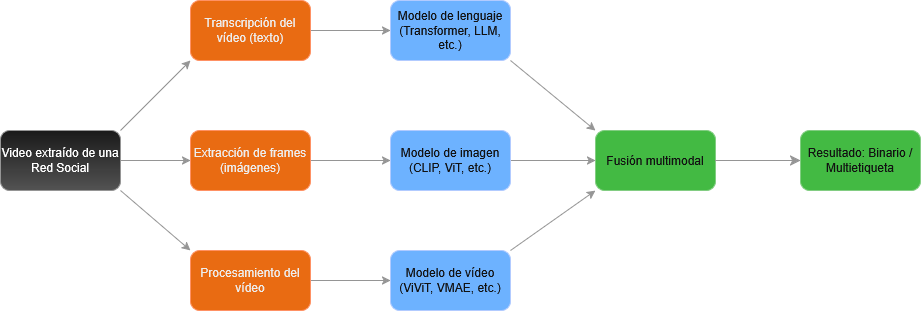
\includegraphics[width=0.9\textwidth]{Figuras/FlujoProcesamientoMultimodal.drawio.png}
    \caption{Flujo de procesamiento multimodal de vídeos (texto + imagen + vídeos)}
    \label{fig:flujo_video}
\end{figure}

Como se ilustra de manera conceptual en la \autoref{fig:flujo_video}, un flujo de procesamiento multimodal estándar divide el contenido original en sus componentes básicos. Cada modalidad es procesada de forma independiente y en paralelo por modelos específicos para extraer sus características intrínsecas. Finalmente, estas representaciones convergen en un módulo de fusión, el cual combina la información para emitir la predicción final. Este esquema teórico sirve como pilar fundamental para el diseño de arquitecturas capaces de analizar el complejo contenido multimedia actual. 

\section{Aprendizaje Profundo}
\label{sec:DeepLearning}
Dentro de la disciplina del aprendizaje automático, el aprendizaje profundo (\textit{Deep Learning}) representa una evolución significativa \cite{goodfellow2016deep}. Esta rama se fundamenta en el uso de redes neuronales artificiales, arquitecturas computacionales inspiradas en cómo el cerebro humano estructura y procesa la información. Al organizar estas neuronas artificiales en múltiples capas sucesivas, el sistema adquiere la capacidad de procesar la información de forma jerárquica, logrando un nivel de abstracción cada vez mayor. A medida que aumenta la profundidad de la red (el número de capas), el algoritmo es capaz de modelar relaciones más complejas y extraer mayor cantidad de información a partir de los datos, incluso si no es perceptible por el ser humano \cite{lecun2015deep}.

\begin{figure}[H]
    \centering
    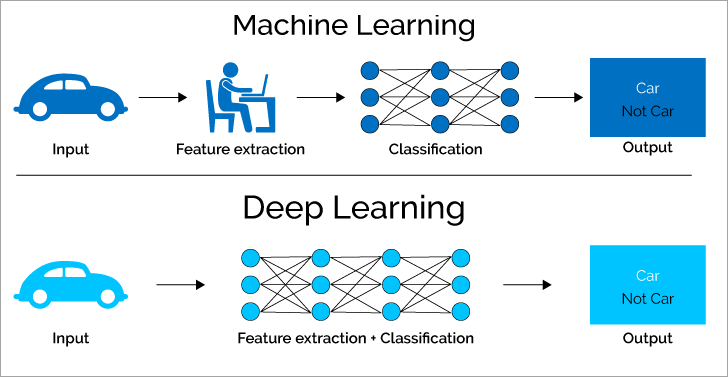
\includegraphics[width=0.9\textwidth]{Figuras/MLvsDL.png}
    \caption{Principal diferencia entre \textit{Machine} y \textit{Deep Learning}}
    \label{fig:MLvsDL}
\end{figure}

La principal diferencia entre el aprendizaje automático clásico y el aprendizaje profundo radica en el proceso de extracción de características (\textit{feature extraction}). Como se ilustra en la \autoref{fig:MLvsDL}, en los algoritmos tradicionales de \textit{Machine Learning}, es necesario que un experto humano o un proceso algorítmico previo diseñe y extraiga manualmente las características relevantes de los datos de entrada para que el clasificador pueda tomar decisiones. Por el contrario, los modelos de \textit{Deep Learning} automatizan este proceso por completo, integrando la extracción de características de forma implícita dentro de la propia arquitectura de la red. Esta capacidad de aprendizaje de extremo a extremo (\textit{end-to-end}) permite al modelo descubrir por sí mismo qué patrones son los más instructivos para resolver la tarea\cite{chollet2021deep}.

En el contexto de este Trabajo de Fin de Máster, el aprendizaje profundo constituye el núcleo técnico del sistema propuesto. Se han empleado modelos basados en arquitecturas profundas, tanto para el procesamiento de la información textual, con modelos \textit{Transformers} y Grandes Modelos de Lenguaje, como para el análisis visual, con modelos \textit{Vision Transformers}

Dado el enorme tamaño de estas arquitecturas y la complejidad matemática que entraña su ajuste, resulta indispensable comprender cómo se lleva a cabo su fase de entrenamiento. El éxito de estos modelos no depende únicamente de su estructura interna, sino de la correcta configuración de los factores que guían su aprendizaje. Por ello, en las siguientes subsecciones se detallan los hiperparámetros, mecanismos de control y conceptos fundamentales que controlan el proceso de entrenamiento. 

\subsection{Epochs y tamaño de lote}
\label{subsec:EpochsBatch}
Durante el proceso de entrenamiento de una red neuronal profunda, el modelo ajusta sus parámetros internos de forma iterativa a medida que procesa la información. El ritmo y el volumen de datos que se procesan en cada actualización de los pesos están regidos por dos hiperparámetros fundamentales de la arquitectura: la época (\textit{epoch}) y el tamaño de lote (\textit{batch size}).

Una época (\textit{epoch}) se define como un ciclo de aprendizaje completo en el que la totalidad del conjunto de datos de entrenamiento pasa a través de la red neuronal, tanto hacia adelante (\textit{forward pass}) para generar las predicciones, como hacia atrás (\textit{backward pass}) para propagar el error. Dado que los algoritmos de optimización basados en el gradiente son iterativos, una sola época rara vez es suficiente para que el modelo minimice el error adecuadamente. Por lo tanto, el entrenamiento exige realizar múltiples épocas. Sin embargo, un número excesivamente alto de épocas puede derivar en un problema de sobreajuste (\textit{overfitting}), donde el modelo comienza a memorizar los datos de entrenamiento perdiendo su capacidad de generalización \cite{prechelt2002early}.

Por otro lado, la cantidad de información que componen los conjuntos de datos actuales (especialmente aquellos con imágenes y vídeos) hace que sea computacionalmente inviable, debido a las limitaciones de memoria de las tarjetas gráficas (\textit{GPU}), procesar todos los ejemplos simultáneamente. Para solucionar esta limitación, el conjunto de entrenamiento se divide en fracciones más pequeñas denominadas lotes (\textit{batches} o \textit{minibatches}). El tamaño de lote determina el número de muestras que la red procesa antes de evaluar el error acumulado y actualizar sus pesos \cite{bengio2012practical}.

La elección del tamaño de lote tiene un impacto directo en la estabilidad y velocidad del entrenamiento. Un lote grande ofrece una estimación muy precisa del gradiente, pero requiere una enorme cantidad de memoria \textit{VRAM}. Por el contrario, un tamaño de lote pequeño introduce cierto ``ruido'' matemático en cada actualización. Curiosamente, este ruido suele ser beneficioso, ya que actúa como un mecanismo de regularización que ayuda a la red a escapar de mínimos locales y a encontrar soluciones que generalizan mejor ante datos nuevos \cite{masters2018revisiting}. 

En el contexto del ajuste fino (\textit{fine-tuning}) de arquitecturas masivas, como los \textit{Transformers} o los \textit{LLMs} empleados en este trabajo, el enorme peso de los modelos obligan a utilizar tamaños de lote muy reducidos. Asimismo, dado que estas redes ya cuentan con un amplio conocimiento adquirido durante su preentrenamiento, el número de épocas necesarias suele ser considerablemente bajo (generalmente entre 3 y 10). Un entrenamiento prolongado en estas condiciones no solo sería ineficiente, sino que podría provocar lo que se conoce como \textit{catastrophic forgetting}, el cual destruiría las representaciones lingüísticas o visuales que el modelo ya había aprendido previamente. 

\subsection{Tasa de aprendizaje y \textit{weight decay}}
\label{subsec:LearningRate}
La tasa de aprendizaje (\textit{learning rate}) es, posiblemente, el hiperparámetro más crítico en la configuración de cualquier algoritmo de optimización basado en el gradiente. Este valor determina el tamaño del paso que da el modelo en el espacio de parámetros durante cada iteración para minimizar la función de pérdida. Su correcta elección tiene un impacto significativo en la convergencia del modelo: si la tasa de aprendizaje es demasiado alta, los saltos en la actualización de los pesos serán desproporcionados, lo que puede provocar que el modelo sobrepase el mínimo óptimo y el entrenamiento se vuelva inestable. Por el contrario, si la tasa es excesivamente baja, la red tardará demasiado tiempo en converger o correrá el riesgo de quedarse estancada en un mínimo local \cite{ruder2016overview}. 

Para complementar el proceso de optimización y mitigar el riesgo de sobreajuste, es práctica común incorporar una técnica de regularización conocida como \textit{weight decay} (decaimiento de pesos). Esta técnica consiste en añadir un término de penalización a la función de pérdida que es proporcional al tamaño de los pesos de la red. De este modo, el algoritmo se ve forzado a mantener los valores de los parámetros lo más pequeños y distribuidos posible. Al evitar que unos pocos pesos adquieran valores desproporcionados, se asume que el modelo resultante es más simple y estable, lo que mejora drásticamente su capacidad para generalizar ante datos no vistos en lugar de memorizar el ruido del conjunto de entrenamiento \cite{krogh1991simple}.

En el ámbito del procesamiento del lenguaje natural y la visión por computador con arquitecturas profundas, ambos conceptos suelen trabajar de la mano mediante optimizadores avanzados como \textit{AdamW}. Al realizar el \textit{fine-tuning} de modelos masivos que ya poseen un conocimiento previo (\textit{Transformers} o \textit{LLMs}), la teoría dictamina el uso de tasas de aprendizaje muy reducidas, a menudo acompañadas de planificadores (\textit{schedulers}) que disminuyen este valor dinámicamente con el tiempo. El uso simultáneo de un \textit{learning rate} bajo y un \textit{weight decay} adecuado garantiza que el modelo se adapte a la nueva tarea de clasificación sin destruir las representaciones que adquirió durante su fase de preentrenamiento \cite{loshchilov2017decoupled}. 

\subsection{Función de pérdida}
\label{subsec:LossFunction}
Durante la fase de entrenamiento, el modelo necesita una métrica cuantitativa que evalúe la precisión de sus predicciones frente a las etiquetas reales del conjunto de datos. Esta métrica es la función de pérdida (\textit{loss function}). Su objetivo matemático es calcular el error cometido en cada predicción, devolviendo un valor que el algoritmo de optimización (mediante \textit{backpropagation}) intentará minimizar iterativamente actualizando los pesos de la red \cite{shalev2014understanding}. En los problemas de clasificación, las funciones de pérdida basadas en la teoría de la información, concretamente en el concepto de entropía, son el estándar. 

Para tareas de clasificación binaria o multiclase, donde las categorías son mutuamente excluyentes (es decir, una entrada solo puede pertenecer a una clase), se emplea la \textbf{Entropía Cruzada} (\textit{Cross-Entropy Loss}). Esta función mide la diferencia entre la distribución predicha por el modelo y la distribución real de las etiquetas. Matemáticamente, penaliza de forma logarítmica las predicciones erróneas que el modelo realiza con alta confianza, forzando al sistema no solo a acertar la clase correcta, sino a hacerlo con la mayor certeza posible \cite{murphy2012machine}. 

Por otro lado, para abordar la tarea de clasificación multietiqueta (donde un mismo registro puede presentar varias categorías de sexismo simultáneamente), el problema se descompone en múltiples clasificaciones independientes. Al tratar cada etiqueta por separado, la entropía cruzada mencionada anteriormente no es aplicable. En su lugar, se utiliza la \textbf{Entropía Cruzada Binaria} (\textit{Binary Cross-Entropy} o \textit{BCE}). Esta variante evalúa la probabilidad de presencia o ausencia de cada etiqueta de manera independiente, permitiendo que el modelo determine si una categoría específica aplica o no a la entrada, sin que dicha decisión afecte a las probabilidades del resto de etiquetas \cite{nam2014large}.

\subsection{Overfitting y técnicas de regularización}
\label{subsec:Overfitting}
Uno de los desafíos más críticos durante el entrenamiento de redes neuronales profundas es el fenómeno conocido como sobreajuste (\textit{overfitting}). Este problema ocurre cuando un modelo es excesivamente complejo en relación con la cantidad de datos de entrenamiento disponibles. En lugar de extraer patrones generales y subyacentes, la red comienza a memorizar el ruido, las anomalías y los detalles específicos del entrenamiento. Como resultado, el modelo alcanza un rendimiento excelente sobre los datos con los que ha sido entrenado, pero fracasa drásticamente al intentar generalizar y predecir sobre datos nuevos o no vistos previamente \cite{ying2019overview}.

Para mitigar el problema y forzar al modelo a aprender representaciones más robustas, se emplean diversas técnicas de regularización. Una de las estrategias más extendidas, que actúa de manera complementaria a la penalización de pesos (\textit{weight decay}) vista en apartados anteriores, es el \textit{Dropout} (abandono). 

El \textit{Dropout} es una técnica de regularización estructural que consiste en desactivar aleatoriamente una proporción de las neuronas de la red, junto con sus respectivas conexiones, durante cada iteración (\textit{forward} y \textit{backward pass}) de la fase de entrenamiento. Al ``apagar'' distintas neuronas en cada paso, se evita que las unidades de la red desarrollen una dependencia mutua excesiva. Esto obliga al modelo a distribuir el aprendizaje, garantizando que la predicción final no dependa de un pequeño grupo de neuronas fuertemente conectadas, sino del conjunto de múltiples sub-redes independientes \cite{srivastava2014dropout}.

En las arquitecturas profundas basadas en mecanismos de atención, como los \textit{Transformers} utilizados en este trabajo tanto para el procesamiento textual como visual, el \textit{Dropout} es un componente fundamental que se encuentra integrado por defecto en el diseño de sus bloques internos. La combinación del \textit{Dropout} arquitectónico con estrategias de optimización regularizadas asegura que el modelo mantenga su capacidad de generalización al adaptarse a la nueva tarea de clasificación.  

\subsection{Early stopping y validación}
\label{subsec:EarlyStopping}
Para monitorizar de forma objetiva el rendimiento de un modelo durante su fase de entrenamiento y detectar a tiempo un posible sobreajuste, resulta imprescindible el uso de un conjunto de validación. Este subconjunto de datos, que se mantiene independiente de las muestras empleadas para actualizar los pesos de la red, permite evaluar iterativamente la capacidad de generalización del modelo. Este proceso se da al finalizar cada época o tras un número determinado de iteraciones y se calcula la función de pérdida y otras métricas de rendimiento sobre este conjunto de validación. 

La observación continua de estas métricas es la base del \textit{early stopping} (parada temprana), una de las técnicas de regularización dinámica más eficaces en el aprendizaje profundo. Esta estrategia consiste en interrumpir el entrenamiento de forma automática antes de completar todas las épocas definidas si se detecta que el rendimiento en validación se estanca o empieza a degradarse, mientras que el error de entrenamiento sigue disminuyendo. Este punto de inflexión es el indicador clave de que el modelo ha dejado de aprender patrones generales y ha empezado a memorizar el conjunto de datos de entrenamiento \cite{bejani2021systematic}.

En la práctica, el \textit{early stopping} se configura mediante un parámetro conocido como paciencia (\textit{patience}), el cual define cuántas evaluaciones sin mejora se permiten antes de detener el proceso. Además de ahorrar valiosos recursos computacionales, esta técnica permite restaurar la configuración de pesos óptima (aquella que obtuvo el mejor resultado en la fase de validación) en lugar de retener los pesos deteriorados de la última época. 

Todos estos elementos analizados en las subsecciones anteriores son fundamentales para diseñar modelos robustos y reproducibles. Además, permiten explicar por qué un modelo ha funcionado mejor que otro cuando se ajustan frente a un problema complejo, más allá de lo que dictan las métricas de evaluación. Como señalan Bergstra y Bengio \cite{bergstra2012random}, el conocimiento de estos hiperparámetros y mecanismos de control es clave para mejorar la eficacia y garantizar el éxito de los modelos de aprendizaje automático.

\section{Procesamiento del Lenguaje Natural}
\label{sec:PLN}
El Procesamiento del Lenguaje Natural (PLN) es una rama de la inteligencia artificial y lingüística computacional que se ocupa de la interacción entre los sistemas informáticos y el lenguaje humano. Su objetivo principal es dotar a las máquinas de la capacidad necesaria para comprender, interpretar, generar y analizar el lenguaje natural, ya sea en formato textual o hablado. En el contexto de este Trabajo de Fin de Máster, el PLN constituye un pilar fundamental para extraer el significado y la intención de los vídeos analizados, permitiendo detectar patrones en el discurso asociados a sesgos de género, misoginia y lenguaje sexista. 

Históricamente, los sistemas de clasificación textual dependían de un preprocesamiento manual y exhaustivo. Este proceso clásico implicaba la aplicación de técnicas morfológicas para limpiar y normalizar los datos, tales como la división del texto en unidades mínimas (\textit{tokenización} por palabras), la eliminación de términos que no tienen una carga semántica dentro de la frase (\textit{stopwords}), la lematización y el truncamiento (\textit{stemming}). Tras esta fase, el texto se transformaba en matrices numéricas basadas en la frecuencia de aparición de los términos (como \textit{TF-IDF} o \textit{Bag-of-Words}). Sin embargo, estos enfoques tradicionales presentaban una limitación estructural crítica: al ignorar el orden de las palabras, se perdía gran parte del contexto y de la semántica subyacente de las frases \cite{li2022survey}.

En la actualidad, la disciplina del PLN ha experimentado una profunda evolución gracias a la adopción de nuevas arquitecturas profundas de aprendizaje automático. Los nuevos modelos, especialmente aquellos basados en la arquitectura \textit{Transformer}, han transformado el paradigma del análisis textual. En lugar de requerir una limpieza léxica manual, estos modelos utilizan tokenizadores de subpalabras (como \textit{Byte-Pair-Encoding}) y proyectan el texto en espacios vectoriales continuos de alta dimensión denominados \textit{embeddings}. Esta representación vectorial permite al modelo conservar de manera simultánea tanto la información sintáctica como la riqueza semántica. Al procesar secuencias de forma bidireccional y contextual, el sistema es capaz de captar matices lingüísticos complejos, como la ironía, el sarcasmo o el doble sentido, elementos que son intrínsecos al lenguaje natural y vitales para detectar el discurso sexista \cite{min2023recent}.

\subsection{Preprocesamiento del texto}
\label{subsec:Preprocesamiento}
Para que un modelo de aprendizaje profundo pueda procesar y extraer valor de la información textual, los datos deben someterse a una fase previa de acondicionamiento. Tal y como se ha mencionado en la sección anterior, aunque las arquitecturas basadas en \textit{Transformers} no requieren técnicas clásicas de limpieza lingüística (como la lematización), sí exigen un proceso de  eliminación de ruido específico del dominio y una tokenización matemática estricta. 

En la fase de experimentación de este trabajo, las transcripciones y textos analizados se han sometido a una tubería de limpieza (\textit{pipeline}) mediante el uso de expresiones regulares. El objetivo ha sido estandarizar el vocabulario (convirtiendo todo el texto a minúsculas) y eliminar aquellos elementos sin valor semántico que introducen ruido en la red. Concretamente, se ha procedido a la eliminación de enlaces web (\textit{URLs}), menciones a otros usuarios, etiquetas de metadatos (\textit{hashtags}), emoticonos (\textit{emojis}) y etiquetas estructurales derivadas de la transcripción de los vídeos (como los prefijos ``AUDIO:'' o ``VIDEO:''). La supresión de estos elementos resulta fundamental para aislar el discurso real y evitar que el modelo dedique recursos a aprender patrones sintácticos irrelevantes para la tarea de clasificación \cite{khurana2023natural}.

Una vez que el texto ha sido limpiado, se aplica el proceso de tokenización. Las nuevas arquitecturas emplean algoritmos de subpalabras, como \textit{Byte-Pair Encoding} (BPE) o \textit{WordPiece}. Estos enfoques son altamente eficientes, ya que conservan las palabras comunes enteras, pero dividen los términos raros, mal escritos o específicos de la jerga de internet en subunidades más pequeñas y conocidas. 

Finalmente, el tokenizador actúa como puente entre el texto y la red neuronal: toma estas subpalabras y las convierte en vectores de identificadores numéricos (\textit{input IDs}). Para garantizar que todas las secuencias adquieran una dimensión matricial uniforme antes de ser procesadas por el modelo, se aplica un proceso de truncamiento (estableciendo una longitud máxima permitida para los registros demasiado largos) y de relleno (\textit{padding}) para los textos más cortos. Adicionalmente, el tokenizador genera estructuras de control, como las máscaras de atención (\textit{attention masks}), las cuales indican al algoritmo qué partes del vector contienen información real y cuáles son simples rellenos. Este formato numérico es el único lenguaje que los modelos de aprendizaje profundo pueden procesar internamente. 

\subsection{Representación del texto}
\label{subsec:Embeddings}
Una vez que el texto ha sido tokenizado, el siguiente reto del PLN es transformar esos identificadores numéricos en un formato que capture el significado lingüístico. Históricamente, esta tarea se realizaba mediante técnicas de extracción de características basadas en frecuencias, como el \textit{Bag-of-Words} o \textit{TF-IDF}. Aunque resultan útiles en algoritmos de aprendizaje automático clásico, estas estrategias generan representaciones dispersas y asumen la independencia entre los términos, fallando a la hora de capturar las relaciones semánticas intrínsecas. 

Para superar estas limitaciones, se introdujeron los \textit{Word Embeddings} o representaciones vectoriales densas. En términos generales, un \textit{Word Embedding} proyecta cada palabra como un vector de números reales en un espacio continuo de alta dimensión, lo que permite cuantificar el contexto de una palabra, así como su similitud semántica y sintáctica, mediante distancias matemáticas.

Uno de los enfoques pioneros en este ámbito fue \textit{Word2Vec}, el cual utiliza redes neuronales poco profundas para aprender representaciones vectoriales mediante dos posibles arquitecturas: \textit{Continuous Bag-of-Words} (\textit{CBOW}), que predice una palabra objetivo a partir de su contexto, o \textit{Skip-Gram}, que realiza la tarea inversa prediciendo el contexto a partir de una palabra principal. Posteriormente, surgieron alternativas como \textit{GloVe} (\textit{Global Vectors for Word Representation}), un modelo que combina las ventajas de los métodos de ventana de contexto local con la factorización matricial global del corpus.  

Sin embargo, estos modelos estáticos presentaban una limitación estructural sin solución: el problema de la polisemia. Dado que algoritmos como \textit{Word2Vec} o \textit{GloVe} precalculan un único vector inamovible para cada término en el vocabulario, son incapaces de distinguir cuándo una misma palabra tiene significados distintos en función del contexto en la oración \cite{jurafsky2014speech}.

Esta debilidad impulsó el desarrollo de la actual generación de representaciones contextuales densas. Las nuevas arquitecturas, en lugar de consultar un diccionario estático de vectores, calculan la representación numérica de cada subpalabra de manera dinámica, analizando simultáneamente toda la secuencia que la rodea. Esta necesidad de contextualización profunda dio lugar a las arquitecturas basadas en mecanismos de atención, las cuales se abordarán en detalle en las siguientes secciones. 

\subsection{Clasificación de texto en PLN}
\label{subsec:ClasificacionPLN}
La clasificación de textos es una de las tareas computacionales más fundamentales dentro del PLN. Su objetivo principal consiste en asignar, de forma automática, una o varias categorías semánticas predefinidas a un fragmento de texto no estructurado. Dependiendo de la complejidad y la naturaleza del problema, los sistemas de clasificación se dividen en tres grandes grupos: clasificación binaria, multiclase y multietiqueta, las cuales ya fueron definidas anteriormente en el apartado \ref{sec:Clasificacion} de esta memoria.

En el contexto de este Trabajo de Fin de Máster, la clasificación de texto se emplea como motor analítico para auditar las transcripciones de los videos seleccionados. El proceso se aborda desde una doble vertiente. En primer lugar, se aplica una clasificación binaria para dictaminar si el contenido expresa algún tipo de lenguaje sexista o misógino. En caso afirmativo, el problema evoluciona hacia un esquema de clasificación más fino y detallado, cuyo objetivo es identificar qué tipos específicos de sesgos, roles de género o violencias discursivas están presentes en el mensaje. 

La relevancia de este desafío tecnológico y social queda patente en las prestigiosas campañas de evaluación competitiva organizadas por congresos internacionales como \textit{IberLEF} o \textit{CLEF}. De hecho, el marco experimental y metodológico desarrollado en este trabajo se fundamenta directamente en la competición \textit{EXIST 2025} (\textit{sEXism Identification in Social neTworks}). 

Concretamente, los modelos implementados en este proyecto dan respuesta a los retos planteados en la \textbf{Tarea 3.1} de dicha competición, centrada en la detección binaria de misoginia en redes sociales, y en la \textbf{Tarea 3.3}, enfocada en la categorización avanzada y el análisis multietiqueta del discurso machista. La participación y adaptación a este tipo de iniciativas garantiza que las soluciones aquí propuestas operan sobre un conjunto de datos estandarizado y contribuyen activamente al estado del arte en la mitigación del discurso de odio en entornos digitales. 

\section{Modelos Avanzados para Texto}
\label{sec:ModelosTexto}
La necesidad de capturar el contenido dinámico y resolver el problema de la polisemia en la representación textual ha propiciado el desarrollo de arquitecturas neuronales de última generación. En esta sección se describen los fundamentos de los modelos basados en mecanismos de atención y su evolución hasta los modernos sistema generativos, los cuales constituyen el núcleo de las tecnologías aplicadas en este trabajo. 

\subsection{Transformers}
\label{subsec:Transformers}
La arquitectura \textit{Transformer}, la cual se puede apreciar en la \autoref{fig:ArquitecturaTransformer}, supuso un cambio de paradigma en el PLN tras ser propuesta en el influyente artículo \textit{Attention is all you need} \cite{vaswani2017attention}. A diferencia de los modelos recurrentes tradicionales, como las Redes Neuronales Recurrentes (RNN) o las redes de memoria a corto-largo plazo (\textit{LSTM}), los \textit{Transformers} prescinden del procesamiento secuencial. Esta característica permite analizar las secuencias de texto en paralelo, lo que acelera drásticamente los tiempos de entrenamiento y facilita la captura de dependencias a muy largo plazo. 

\begin{figure}[H]
    \centering
    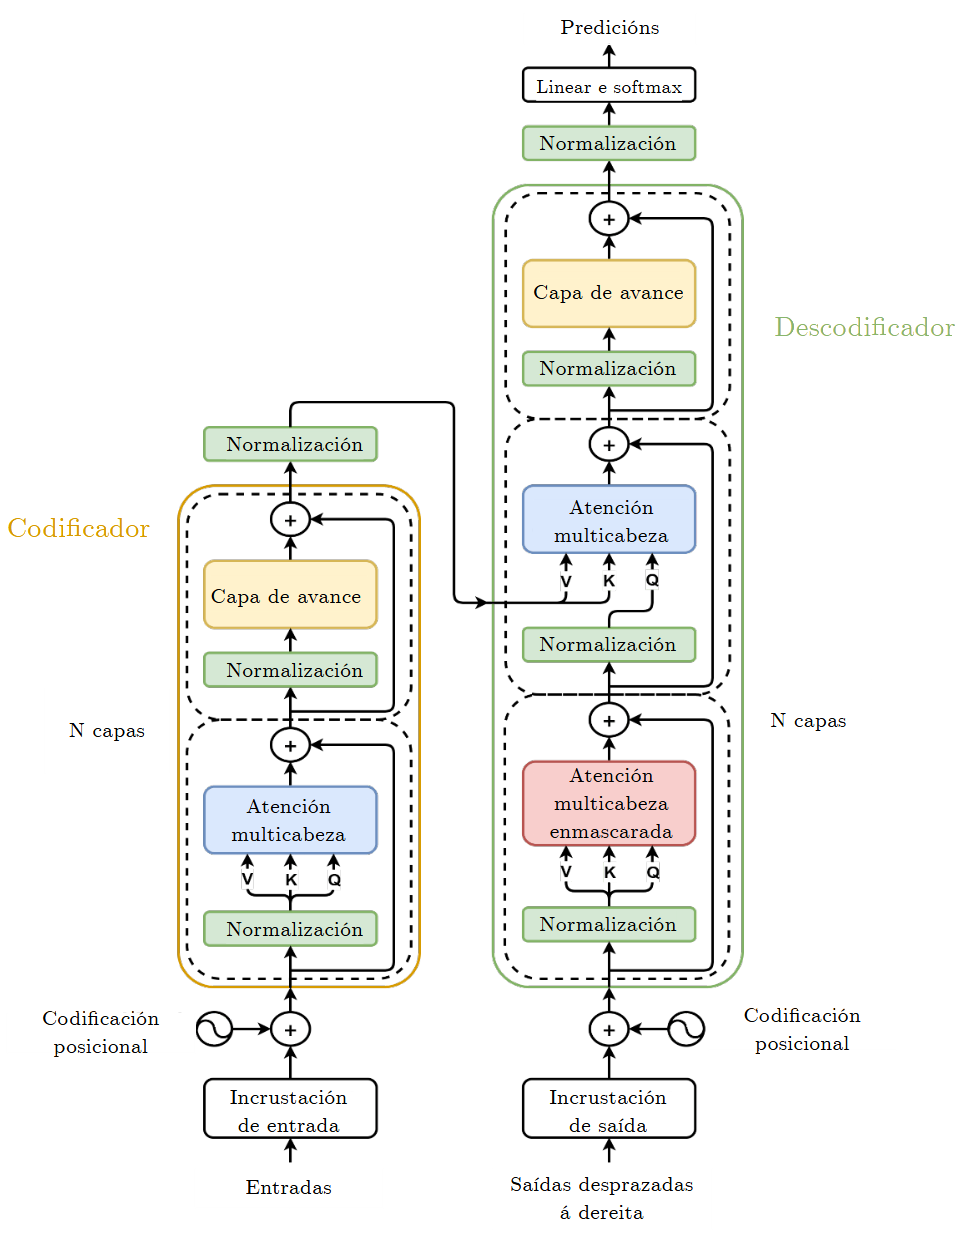
\includegraphics[width=0.9\textwidth]{Figuras/ArquitecturaTransformer.png}
    \caption{Arquitectura de los modelos \textit{Transformers}}
    \label{fig:ArquitecturaTransformer}
\end{figure}

El pilar de esta arquitectura es el mecanismo de autoatención (\textit{self-attention}), cuyo funcionamiento se ejemplifica gráficamente en la \autoref{fig:MecanismoAtencion}. Este mecanismo relaciona diferentes posiciones de una simple secuencia para computar una representación global de la misma. Matemáticamente, asigna una consulta (\textit{query}) y un conjunto de pares clave-valor (\textit{key-value}) a una salida, calculando pesos que determinan la importancia relativa de cada palabra respecto a las demás dentro de la misma oración.

\begin{figure}[H]
    \centering
    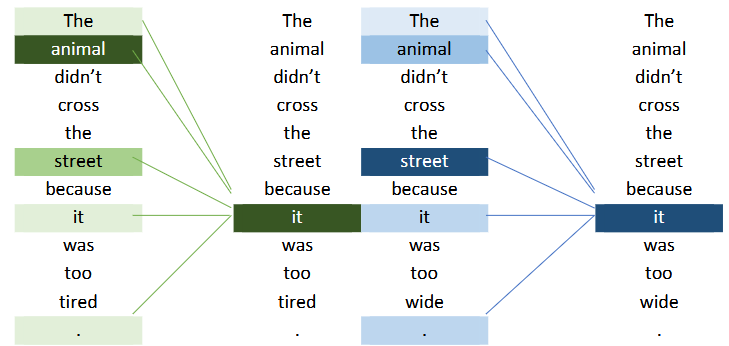
\includegraphics[width=0.9\textwidth]{Figuras/MecanismosAtencionTransformers.png}
    \caption{Ejemplo de funcionamiento del mecanismo de atención}
    \label{fig:MecanismoAtencion}
\end{figure}

Esta innovación dio lugar a una nueva generación de modelos de lenguaje preentrenados fundamentados en la codificación bidireccional, siendo \textit{BERT} (\textit{Bidirectional Encoder Representations from Transformers}) \cite{devlin2018bert} el exponente clásico. Este necesita de las entradas que se muestran en la \autoref{fig:EncoderBERT}. \textit{BERT} es capaz de aprender el contexto de una palabra observando su secuencia antecesora y predecesora de manera simultánea. Posteriormente, surgieron optimizaciones robustas como \textit{RoBERTa} (\textit{Robustly Optimized BERT Approach}) \cite{liu2019roberta}, que mejora el rendimiento eliminando la predicción de la siguiente oración durante el preentrenamiento, utilizando secuencias más largas e introduciendo un enmascaramiento dinámico de los datos. 

\begin{figure}[H]
    \centering
    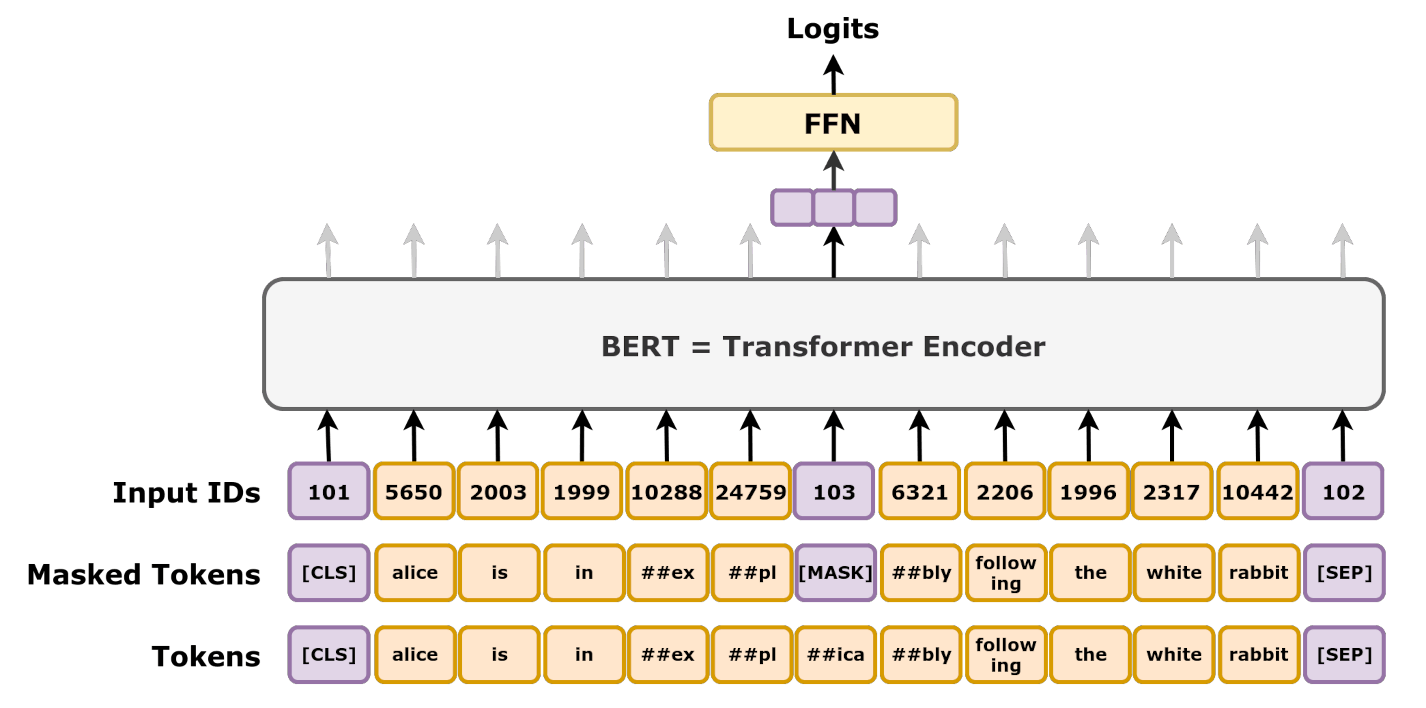
\includegraphics[width=0.9\textwidth]{Figuras/BERTEncoder.png}
    \caption{Entradas necesarias para el codificador de \textit{BERT}}
    \label{fig:EncoderBERT}
\end{figure}

\subsubsection*{Modelos implementados en este trabajo}
\label{subsubsec:ModelosTransformers}
Para abordar la complejidad de esta tarea y asegurar una evaluación exhaustiva, en el desarrollo empírico de este Trabajo de Fin de Máster se ha implementado una amplia batería de arquitecturas discriminativas basadas en \textit{Transformers}, adaptadas a diferentes dominios lingüísticos:
\begin{itemize}
    \item \textbf{Modelos Multilingües}: Se han utilizado \texttt{mmBERT}, \texttt{xlm-roberta-base} y \texttt{TwHIN-BERT}, idóneos para captar estructuras semánticas universales y transferir conocimiento entre idiomas.
    \item \textbf{Modelos específicos para Español}: Se han evaluado \texttt{BETO}, \texttt{BERTin} y \texttt{RoBERTuito}, siendo este último optimizado para el lenguaje informal de redes sociales. 
    \item \textbf{Modelos específicos para Inglés}: Se ha experimentado con \texttt{RoBERTa-Base}, \texttt{BERTweet} (preentrenado en mensajes cortos y jerga digital) y \texttt{Electra-base-discriminator} (que introduce un paradigma de reemplazo de tokens más eficiente computacionalmente). 
\end{itemize}


\subsection{Modelos Generativos de Lenguaje (\textit{LLMs})}
\label{sec:LLMs}
Paralelamente a la consolidación de modelos discriminativos como \textit{BERT}, la evolución del aprendizaje profundo ha propiciado la explosión de los Modelos Generativos de Lenguaje (\textit{Large Language Models}) \cite{zhao2023survey}. A diferencia de los enfoques anteriores, los cuales están entrenados para comprender y clasificar, los \textit{LLMs} utilizan arquitecturas autorregresivas fundamentadas habitualmente en la parte decodificadora del \textit{Transformer}. Su objetivo matemático principal es predecir el siguiente token de una secuencia para generar texto altamente coherente y contextualizado.

Modelos como \texttt{GPT-3}, \texttt{GPT-4}, \texttt{LLaMA} o \texttt{PaLM} se entrenan sobre volúmenes masivos de datos no estructurados. Gracias a este vasto conocimiento subyacente, han demostrado capacidades de generalización sorprendentes. Una de las ventajas más potentes de los \textit{LLMs} es su capacidad para ejecutar tareas supervisadas a través del diseño de instrucciones o \textit{prompting}. Existen tres estrategias principales de aplicación: 
\begin{itemize}
    \item \textbf{Zero-shot}: El modelo realiza la tarea directamente con una única instrucción, sin recibir ejemplos previos. Es idóneo cuando se busca rapidez o no se dispone de datos etiquetados. 
    \begin{itemize}
        \item \textit{Ejemplo}: ``¿La siguiente transcripción de un vídeo de TikTok a texto contiene lenguaje sexista? Texto: `Las mujeres no sirven para liderar proyectos.' Responde únicamente Sí o No''
    \end{itemize}
    \item \textbf{Few-shot}: Se incluyen varios ejemplos demostrativos dentro de la propia instrucción para que el modelo identifique el patrón deseado antes de emitir su respuesta.
    \begin{itemize}
        \item \textit{Ejemplo}:
        \begin{itemize}
            \item Texto de ejemplo: ``Todos merecemos las mismas oportunidades.'' $\rightarrow$ No sexista.
            \item Texto de ejemplo : ``Las chicas son demasiado emocionales para los negocios.'' $\rightarrow$ Sexista.
            \item Texto nuevo: ``Ellas deberían quedarse cuidando la casa.'' $\rightarrow$ El modelo infiere y dictamina que es Sexista.
        \end{itemize}
    \end{itemize}
    \item \textbf{Fine-tuning (Ajuste fino)}: Consiste en entrenar los pesos del modelo preentrenado utilizando un conjunto de datos específicos del dominio. Aunque requiere mayores recursos computacionales, suele ofrecer un rendimiento superior y constante.  
\end{itemize}

\subsubsection*{Aplicación práctica en este trabajo: \textit{PEFT} y \textit{QLoRA}}
\label{subsubsec:ModelosLLMs}
En el marco experimental de este proyecto se ha apostado firmemente por el ajuste fino. Sin embargo, debido al masivo número de parámetros de los \textit{LLMs} modernos, el reentrenamiento completo resulta computacionalmente inviable. Para solucionar este obstáculo, se ha implementado una técnica \textbf{QLoRA} (\textit{Quantized Low-Rank Adaptation}) \cite{dettmers2023qlora} sobre tres modelos generativos de última generación: \texttt{Mistral-7B-Instruct-v0.3}, \texttt{meta-llama/Llama-3.1-8B-} \texttt{Instruct} y \texttt{google/gemma-2-2b-it}. Esta metodología ha permitido cuantizar los pesos base de los modelos a una precisión de 4 bits, congelarlos, y entrenar únicamente matrices de bajo rango insertadas en las proyecciones matemáticas de atención. 

Para adaptar estos modelos a la clasificación binaria de las transcripciones de vídeo, se han desarrollado dos estrategias arquitectónicas distintas: 
\begin{itemize}
    \item \textbf{Enfoque Discriminativo (\textit{Sequence Classification})}: En los modelos \textit{Mistral} y \textit{Gemma}, se sustituyó la cabeza de modelado de lenguaje original por una capa lineal de clasificación pura (\texttt{AutoModelForSequenceClassification}), ajustando los pesos de esta nueva capa (\texttt{score}) para extraer directamente la probabilidad matemática de que el texto contenga lenguaje misógino.
    \item \textbf{Enfoque Generativo Autorregresivo (\textit{Causal LM})}: En el modelo de la familia \textit{LLaMa}, se mantuvo la arquitectura generativa intacta (\texttt{AutoModelForCausalLM}). El ajuste fino se realizó formateando las instrucciones de entrada (\textit{prompts}) para forzar al modelo a predecir y autocompletar exclusivamente un token de clasificación (``YES'' para contenido sexista o ``NO'' para contenido no sexista) mediante un optimizador supervisado (\texttt{SFTTrainer}).
\end{itemize}

\subsubsection*{Ventajas y limitaciones de la clasificación con \textit{LLMs}}
\label{subsubsec:VentajasYLimitacionesLLMs}
La adopción de estas arquitecturas masivas para tareas de clasificación del discurso de odio es una tendencia en alza, aunque presenta características contrastadas: 
\begin{itemize}
    \item \textbf{Ventajas}: Permiten aprovechar un conocimiento semántico universal y el contexto general del mundo, se adaptan rápidamente a nuevas definiciones de categorías, y alcanzan un nivel de comprensión profundo de la ironía o el sarcasmo. 
    \item \textbf{Limitaciones}: Su naturaleza generativa los hace susceptibles a sufrir alucinaciones o generar salidas inconsistentes si no se ajustan correctamente (como ocurre con la modalidad \textit{zero-shot}), exhiben una alta sensibilidad al diseño de la instrucción (\textit{prompt}) y conllevan un coste computacional elevado para inferencias masivas.
\end{itemize}

\section{Modelos Avanzados para Visión Estática (Imágenes)}
\label{sec:ModelosAvanzadosParaVisionEstatica}
De manera análoga a la evolución experimentada en el PLN, la visión por computador ha sufrido una profunda transformación en los últimos años. Una de las estrategias más eficientes para el análisis de vídeo consiste en eludir el altísimo coste computacional de las arquitecturas tridimensionales (\textit{3D-CNNs}) \cite{carreira2017quo} extrayendo secuencias de fotogramas clave y tratándolos como imágenes estáticas independientes. Para procesar estas imágenes, el estado del arte actual se divide en dos grandes enfoques según su topología.

\subsection{\textit{Vision Transformers} (\textit{ViT}) y variantes jerárquicas}
\label{subsec:ViT}
Inspirados por el abrumador éxito de los mecanismos de autoatención en el texto conseguido gracias a los \textit{Transformers}, en 2020 se introdujeron los \textit{Vision Transformers} (\textit{ViT}) \cite{dosovitskiy2020image}, demostrando que la dependencia de las redes convolucionales tradicionales no era estrictamente necesaria para tareas de visión complejas. 

La arquitectura \textit{ViT} divide la imagen original en una cuadrícula de pequeños parches (por ejemplo, 16x16 píxeles). Tal y como se muestra en la \autoref{fig:ViT} cada parche es aplanado y proyectado linealmente para formar un vector, operando funcionalmente como si fuera un \textit{token} o palabra en una frase. Tras añadir \textit{embeddings} posicionales para retener la información espacial, esta secuencia de parches se introduce directamente en el codificador de un \textit{Transformer} estándar. Al procesar las relaciones globales entre todos los parches mediante la autoatención, \textit{ViT} es capaz de captar un contexto visual integral desde las primeras capas. 

\begin{figure}[H]
    \centering
    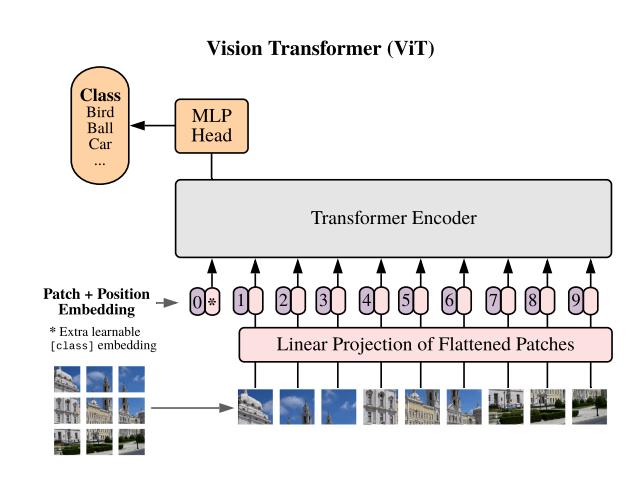
\includegraphics[width=0.9\textwidth]{Figuras/ViT.png}
    \caption{Arquitectura de un \textit{ViT}}
    \label{fig:ViT}
\end{figure}

A pesar de su éxito, \textit{ViT} presenta una complejidad computacional cuadrática respecto a la resolución de la imagen. Para solventar este problema, surgieron variantes como \textit{Swin Transformer} (\textit{Shifted Window Transformer}) \cite{liu2021swin}. Esta arquitectura jerárquica computa la atención de manera local dentro de ventanas no superpuestas que se van desplazando entre capas, lo que otorga mayor flexibilidad y eficiencia a la hora de procesar distintas escalas visuales. 

\subsection{Redes Neuronales Convolucionales Modernas (\textit{ConvNeXt})}
\label{subsec:convnext}
El auge de los \textit{ViT} llevó a repensar y modernizar el diseño clásico de las Redes Neuronales Convolucionales (\textit{CNNs}). Investigadores de \textit{Facebook} y de la Universidad de California propusieron \textit{ConvNeXt} \cite{liu2022convnet}, una arquitectura puramente convolucional construida a partir de una red residual estándar (\textit{ResNet}) \cite{he2016deep}, pero incorporando las decisiones de diseño que hicieron triunfar a los \textit{Transformers}.

Entre estas mejoras estructurales destacan el uso de tamaños de filtro (\textit{kernel}) más grandes, la sustitución de la normalización por lotes (\textit{Batch Normalization}) por la normalización de capas (\textit{Layer Normalization}), y el uso de funciones de activación más suaves. El resultado es una red que sostiene la propia eficiencia computacional de las \textit{CNNs}, pero que logra igualar o incluso superar la precisión de arquitecturas basadas en mecanismos de atención como \textit{Swin Transformer}.

\subsection{Agregación temporal para clasificación de vídeo}
\label{subsec:inferenciaViT}
Cuando estas arquitecturas de imagen estática se aplican a la clasificación de vídeos (como es el caso de este trabajo), el sistema emite una predicción matemática probabilística de forma aislada para cada fotograma extraído de la secuencia temporal. Dado que el objetivo final es emitir un único veredicto global para todo el archivo multimedia, resulta teóricamente indispensable aplicar heurísticas de agregación o \textit{pooling}.

En la literatura científica, las estrategias de consolidación más habituales para agrupar estas predicciones independientes son: 
\begin{itemize}
    \item \textbf{Max-Pooling (sensibilidad máxima)}: Consiste en evaluar el valor máximo de probabilidad de toda la secuencia. Entonces, si un solo fotograma contiene evidencias claras que superan el umbral de activación, todo el vídeo hereda dicha clasificación. Es ideal para detectar anomalías o infracciones breves pero críticas. 
    \item \textbf{Average-Pooling (Promedio continuo)}: Se calcula la media aritmética de las probabilidades de todos los fotogramas. Esta técnica exige que el contenido mantenga un nivel de confianza sostenido a lo largo del tiempo para influir en el veredicto final. 
    \item \textbf{Majority Vote (votación por mayoría)}: Cada fotograma emite un voto discreto (positivo o negativo). El vídeo adopta la clasificación que haya obtenido si supera un umbral definido previamente (lo que se consideraría como mayoría). Es una estrategia altamente robusta frente a fotogramas ruidosos, corruptos o atípicos (\textit{outliers}). 
\end{itemize}

Los detalles específicos sobre la selección de estos modelos, el volumen de fotogramas extraídos por vídeo y la implementación práctica de estas métricas de agregación se detallarán exhaustivamente en el capítulo correspondiente a la metodología experimental.  

\section{Modelos Avanzados para Visión Temporal (Vídeos)}
\label{sec:ModelosAvanzadosParaVisionTemporal}
Aunque el análisis basado en la extracción de fotogramas estáticos reduce drásticamente la carga computacional, esta metodología descarta una dimensión fundamental de los archivos multimedia: la progresión temporal. Para comprender acciones complejas, ironías o comportamientos que se desarrollan a lo largo de un clip, los sistemas de inteligencia artificial deben ser capaces de modelar conjuntamente el espacio (los píxeles en un instante dado) y el tiempo (la evolución de dichos píxeles a través de los fotogramas). En esta sección se abordan las arquitecturas modernas diseñadas para procesar el vídeo como un volumen continuo. 

\subsection{Adaptación de la Arquitectura \textit{Transformer} al Vídeo}
\label{subsec:AdaptacionDeLaArquitecturaTransformerAlVideo}
La aplicación directa del mecanismo de \textit{self-attention} a todos los píxeles de todos los fotogramas de un vídeo resulta computacionalmente inviable, ya que la complejidad matemática crece de forma cuadrática respecto a la longitud de la secuencia de entrada. Para solucionar este enorme cuello de botella, la literatura científica ha propuesto adaptaciones eficientes que extienden el éxito del \textit{ViT} al ámbito tridimensional.

\begin{figure}[H]
    \centering
    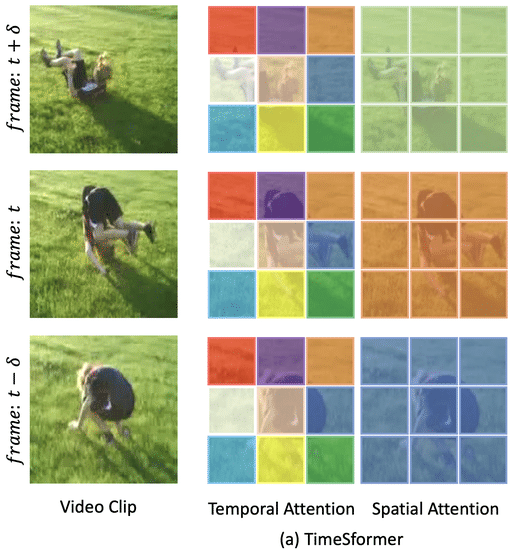
\includegraphics[width=0.6\textwidth]{Figuras/TimeSFormer.png}
    \caption{Ilustración de los mecanismos de atención de un \textit{TimeSformer}}
    \label{fig:TimeSFormer}
\end{figure}

Dentro de este campo, destacan dos enfoques arquitectónicos fundamentales implementados en el desarrollo de este trabajo: 
\begin{itemize}
    \item \textbf{\textit{TimeSformer} (\textit{Time-Space Transformer})}: Propuesto por investigadores de \textit{Facebook} \cite{bertasius2021space}, este modelo resuelve el problema de la explosión paramétrica mediante la \textbf{atención dividida}. En lugar de comparar cada parche con todos los demás parches del vídeo simultáneamente, \textit{TimeSformer} realiza el cálculo en dos pasos: primero aplica una atención puramente espacial (comparando los parches dentro de un mismo fotograma) y, a continuación, aplica una atención puramente temporal (comparando el mismo parche exclusivamente con sus homólogos en los fotogramas anteriores y posteriores), tal y como se puede observar en la \autoref{fig:TimeSFormer}. 
    \item \textbf{\textit{ViViT} (\textit{Video Vision Transformer})}: Desarrollado por investigadores de \textit{Google} \cite{arnab2021vivit}, es la evolución directa del \textit{ViT} estático. Su mayor innovación es el cambio en la forma de extraer las características iniciales: en lugar de dividir la imagen en parches bidimensionales (2D), \textit{ViViT} extrae lo que se conoce como \textbf{\textit{Tubelets}} o tubos tridimensionales. Como se puede apreciar en la \autoref{fig:ViViT}, estos tubos agrupan un bloque de píxeles que atraviesa varios fotogramas consecutivos, permitiendo a la red capturar dinámicas espaciotemporales (como la dirección y la velocidad de un movimiento) desde la primera capa del codificador.  
\end{itemize}

\begin{figure}[H]
    \centering
    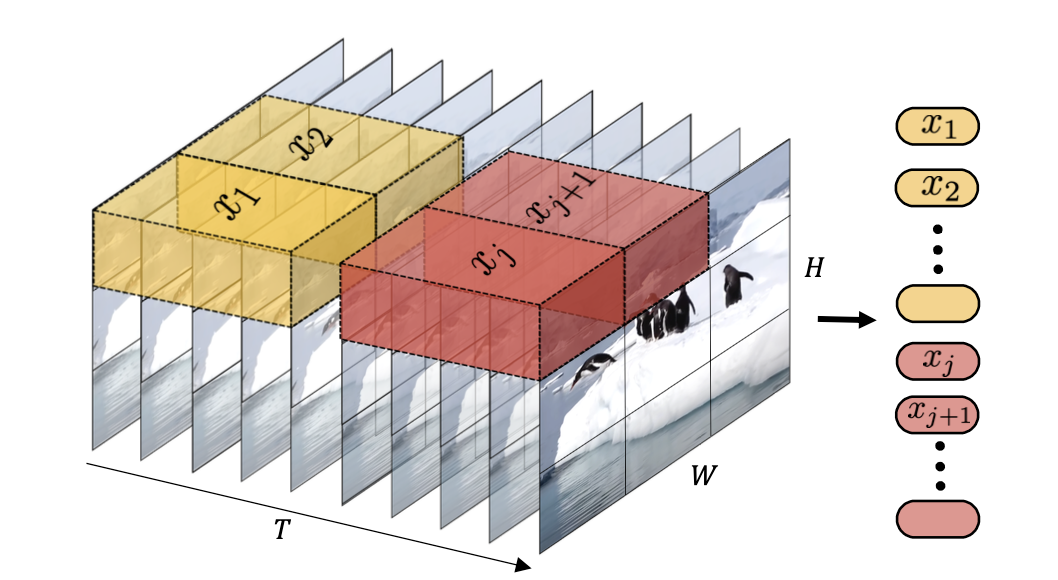
\includegraphics[width=0.9\textwidth]{Figuras/ViViT.png}
    \caption{Representación de los \textit{Tubelets} de los \textit{ViViT}}
    \label{fig:ViViT}
\end{figure}

\subsection{Enfoques Basados en Autoencoders Enmascarados}
\label{subsec:EnfoquesBasadosEnAutoencodersEnmascarados}
Paralelamente a las adaptaciones topológicas del \textit{Transformer}, el entrenamiento de modelos de vídeo ha experimentado una gran revolución gracias a las técnicas de aprendizaje autosupervisado. El principal reto del aprendizaje en vídeo es la \textbf{redundancia de la información}: dos fotogramas consecutivos suelen ser casi idénticos, lo que provoca que las redes neuronales colapsen o memoricen atajos visuales en lugar de aprender características profundas. 

Para combatir este fenómeno, surgieron modelos como \textbf{\textit{VideoMAE}} (\textit{Video Masked Autoencoders}) \cite{tong2022videomae}, una arquitectura inspirada en los métodos de entrenamiento con enmascaramiento nacidos en el PLN (como \textit{BERT}).

El funcionamiento de \textit{VideoMAE} se basa en un paradigma de reconstrucción extrema. Tal y como podemos observar en la \autoref{fig:videoMAE}, el modelo toma un volumen de vídeo (dividido en cubos espaciotemporales) y \textbf{oculta deliberadamente hasta el 90\% de la información}. El codificador (\textit{encoder}) solo procesa el 10\% de los parches visibles, y posteriormente, un decodificador (\textit{decoder}) es forzado a reconstruir todos los píxeles originales que faltan. Este nivel de enmascaramiento tan agresivo impide que la red se apoye en la redundancia temporal de los píxeles vecinos, obligándola a desarrollar una comprensión semántica de muy alto nivel sobre la física, el movimiento y la estructura de los objetos que aparecen en pantalla.

\begin{figure}[H]
    \centering
    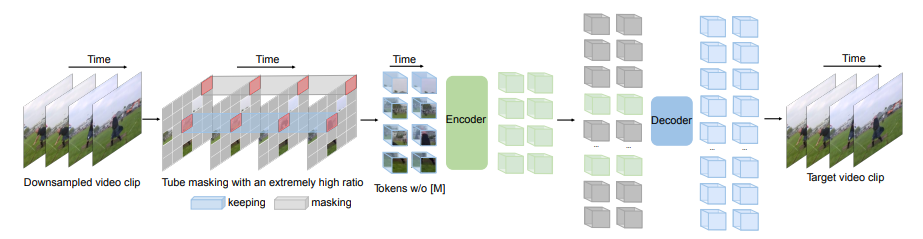
\includegraphics[width=0.9\textwidth]{Figuras/videoMAE.png}
    \caption{Arquitectura de \textit{VideoMAE}}
    \label{fig:videoMAE}
\end{figure}

\section{Aprendizaje por Transferencia}
\label{sec:TransferLearning}
El aprendizaje por transferencia (\textit{Transfer Learning}) ha revolucionado el desarrollo de la inteligencia artificial, consolidándose como el enfoque estándar en el PLN, la Visión Artificial y el aprendizaje multimodal \cite{pan2009survey}. Este paradigma consiste en reutilizar el conocimiento previamente adquirido por un modelo computacional al resolver una tarea genérica (generalmente entrenado con volúmenes de datos masivos) para aplicarlo a la resolución de una tarea nueva y específica, la cual suele disponer de una cantidad mucho menor de datos etiquetados. 

Históricamente, el desarrollo de sistemas de aprendizaje profundo exigía inicializar los pesos de las redes neuronales de forma aleatoria y entrenarlas desde cero, un proceso que requería un enorme coste computacional y bases de datos gigantescas para evitar el sobreajuste. El aprendizaje por transferencia elimina esta barrera: en lugar de aprender a extraer características desde la nada, se parte de un modelo preentrenado que ya posee representaciones universales del lenguaje (como es el caso de \textit{BERT}, \textit{RoBERTa} o \textit{GPT}) o de las imágenes \cite{qiu2020pre}. Este conocimiento base se transfiere y se refina para la nueva tarea, permitiendo democratizar el uso de modelos masivos y obtener resultados competitivos con tiempos de entrenamiento significativamente menores. 

\subsection{Fine-tuning y optimización de hiperparámetros}
\label{subsec:FineTuning}
Dentro del aprendizaje por transferencia, la estrategia de adaptación más utilizada y efectiva es el ajuste fino o \textit{fine-tuning}. Este proceso, popularizado en el PLN por enfoques como ULMFiT \cite{howard2018universal}, consiste en tomar la arquitectura de un modelo preentrenado, añadirle una nueva capa de salida orientada a la tarea específica a resolver (por ejemplo, una capa de clasificación binaria) y ajustar los pesos internos de toda la red, o de una parte de ella, utilizando un conjunto de datos propio del dominio.

Sin embargo, la literatura científica ha demostrado que modelos masivos como \textit{BERT} o \textit{RoBERTa} son altamente inestables y sensibles durante esta fase de adaptación \cite{dodge2020fine}. Para que el \textit{fine-tuning} sea exitoso y el modelo no ``olvide'' catastróficamente lo que aprendió en su preentrenamiento, resulta imprescindible realizar un proceso de \textbf{Optimización de Hiperparámetros} (\textbf{\textit{HPO}}). A nivel teórico, existen diversas estrategias para explorar el espacio de hiperparámetros: desde la búsqueda exhaustiva (\textit{Grid Search}) y la búsqueda aleatoria (\textit{Random Search}), hasta métodos avanzados como la optimización bayesiana, que modela probabilísticamente  el rendimiento de combinaciones pasadas para guiar la búsqueda de forma inteligente \cite{akiba2019optuna}.

Durante este proceso de optimización, las variables de configuración que rigen cómo aprende el algoritmo son determinantes y se dividen en:  
\begin{itemize}
    \item Por un lado, parámetros estructurales como el \textit{Learning Rate}, \textit{Weight Decay} y \textit{Epochs}, que ya fueron definidos en la \autoref{subsec:LearningRate} y \autoref{subsec:EpochsBatch} respectivamente. 
    \item Por otro lado tenemos:
    \begin{itemize}
        \item \textbf{Calentamiento (\textit{Warmup})}: Consiste en iniciar el entrenamiento con una tasa de aprendizaje cercana a cero y aumentarla gradualmente durante un porcentaje inicial de los pasos, evitando actualizaciones bruscas que desestabilicen el modelo.
        \item \textbf{Planificador de la tasa (\textit{LR Scheduler})}: Algoritmo que ajusta de forma dinámica la tasa de aprendizaje a medida que avanzan las épocas (por ejemplo, reduciéndola de forma lineal o mediante una curva coseno). 
    \end{itemize}
\end{itemize}

\subsubsection*{Estrategias avanzadas de optimización}
\label{subsubsec:EstrategiasAvanzadasDeOptimizacion}
En la práctica empírica de entrenamiento de modelos masivos como los de visión estática y los de visión temporal, la combinación de estos hiperparámetros ha dado lugar a estrategias de ajuste específicas: 
\begin{itemize}
    \item \textbf{Estrategia conservadora o \textit{Slow Cooker}}: Consiste en someter al modelo a un entrenamiento prolongado (mayor número de épocas) utilizando un \textit{learning rate} muy bajo y un \textit{weight decay} excepcionalmente alto (regularización agresiva). Se acompaña de un periodo de \textit{warmup} prolongado. Es ideal para que el modelo aprenda patrones complejos y sutilezas en conjuntos de datos difíciles sin memorizarlos. 
    \item \textbf{Simulación de lotes masivos (\textit{Gradient Accumulation})}: La memoria de las tarjetas gráficas (\textit{VRAM}) suele limitar el tamaño del lote de datos (\textit{batch size}) que se puede procesar simultáneamente. Para lograr gradientes matemáticamente estables como los que ofrecería un lote masivo, se acumulan los gradientes de varios lotes pequeños durante múltiples iteraciones antes de ejecutar la actualización de los pesos. 
    \item \textbf{Ajuste agresivo o \textit{Sprint Final}}: Se utiliza una combinación de \textit{learning rate} y regularización moderadas, pero aplicando un planificador tipo coseno (\textit{Cosine Scheduler}). Tras un calentamiento inicial, la tasa de aprendizaje se mantiene estable para luego decaer rápida y suavemente hacia el final, exprimiendo el máximo rendimiento de la red en las últimas iteraciones.
\end{itemize}

\section{Ensemble de Modelos y Fusión multimodal}
\label{sec:Ensemble}
En el ámbito del aprendizaje automático, la técnica de \textit{ensemble} (conjunto de modelos) consiste en combinar las predicciones de múltiples algoritmos diversos para generar una única decisión final más robusta, estable y precisa \cite{sagi2018ensemble}. La premisa matemática detrás de esta técnica es que, al agregar diferentes perspectivas, los errores individuales de cada modelo se compensan mutuamente, reduciendo la varianza y mitigando los sesgos específicos de cada arquitectura. 

En el contexto del análisis del discurso de odio en redes sociales, la información es inherentemente multimodal. Un vídeo no se compone de una única fuente de información, sino que abarca la transcripción textual del audio, la composición visual de sus fotogramas estáticos y la evolución temporal de sus movimientos. 

\subsection{Ventajas de los \textit{Transformers} en tareas multimodales}
\label{subsec:VentajaDeLosTransformersEnTareasMultimodales}
La capacidad de los \textit{Transformers} y de las modernas arquitecturas convolucionales para manejar secuencias de cualquier tipo y capturar dependencias a largo plazo los convierte en herramientas extremadamente potentes para tareas multimodales. En lugar de depender de un único modelo monolítico que intente comprender todo a la vez, la tendencia actual se orienta a utilizar arquitecturas expertas dedicadas que procesan el texto, la imagen y el vídeo en paralelo, combinando su información a posteriori para realizar predicciones conjuntas. Este enfoque permite capturar con una altísima precisión las relaciones y contradicciones entre lo que se dice en la transcripción de un vídeo y lo que se muestra en su componente visual. 

\subsection{Fusión Temprana vs Fusión Tardía}
\label{subsec:FusionTempranaVsFusionTardia}
A nivel teórico, la integración de múltiples modalidades de datos se divide principalmente en dos tipos \cite{baltrusaitis2018multimodal}: 
\begin{itemize}
    \item \textbf{Fusión Temprana (\textit{Early Fusion})}: Los datos o características extraídas de diferentes modalidades se combinan en las primeras etapas de la red neuronal, creando un vector unificado que es procesado por un único clasificador final. Aunque permite que el modelo aprenda interacciones cruzadas desde el principio, es computacionalmente muy costoso y propenso al \textit{overfitting} si una modalidad domina sobre las demás.
    \item \textbf{Fusión Tardía (\textit{Late Fusion})}: Cada modalidad es procesada por un modelo experto independiente hasta generar una predicción final (una probabilidad matemática). Posteriormente, estas probabilidades aisladas se combinan mediante algoritmos estadísticos para emitir el veredicto definitivo. 
\end{itemize}

En la práctica empírica y en las competiciones de Ciencia de Datos, el \textbf{\textit{late fusion} mediante predicción estática} se ha estandarizado como la metodología más eficiente. Al separar la fase de inferencia de la fase de combinación, esta técnica permite ajustar y recalcular el peso de cada modelos miles de veces en cuestión de milisegundos, sin necesidad de reprocesar repetidamente la costosa extracción de características a través de las tarjetas gráficas (\textit{VRAM}).

\subsubsection*{Promedio Ponderado (\textit{Weighted Average})}
\label{subsubsec:PromedioPonderado}
Una de las estrategias matemáticas más utilizadas en la fusión tardía es el promedio ponderado. En este método, a la probabilidad emitida por cada modelo experto se le asigna un peso específico ($w$) que refleja su nivel de fiabilidad o importancia empírica en el conjunto del sistema. Matemáticamente, la probabilidad final unificada se calcula del siguiente modo: 

\begin{equation}
    P_{final} = (w_{texto} \cdot P_{texto}) + (w_{imagen} \cdot P_{imagen}) + (w_{video} \cdot P_{video})
    \label{eq:PesosEnsemble}
\end{equation}

Sujeto a la restricción de que la suma de todos los pesos sea exactamente 1. Los valores óptimos de estos pesos no se definen arbitrariamente, sino que se descubren mediante algoritmos de búsqueda y validación cruzada que evalúan qué combinación exacta maximiza las métricas de rendimiento sobre un conjunto de datos estático. 

\section{Subjetividad en la anotación de los datos}
\label{sec:SubjetividadEnLaAnotacionDeLosDatos}
En los sistemas de aprendizaje automático tradicionales, se asume que existe una única ``verdad absoluta'' para cada conjunto de datos. Sin embargo, en tareas vinculadas al PLN que involucran un alto componente subjetivo, como la detección del discurso de odio, el sexismo o la toxicidad, esta premisa se desvanece. La percepción de un mensaje como ofensivo está intrínsecamente ligada a la sensibilidad, el contexto cultural y las experiencias vitales de la persona que lo evalúa. Por tanto, el desacuerdo entre los anotadores humanos no debe considerarse necesariamente como un ``ruido'' o un error en el conjunto de datos, sino como una señal valiosa que refleja la ambigüedad real del lenguaje humano. 

\subsection{Aprendizaje con Desacuerdo (Learning with Disagreement)}
\label{subsec:LWD}
Para gestionar esta multiplicidad de opiniones en la fase de entrenamiento de los modelos, el estado del arte ha evolucionado desde el consenso estricto hacia el \textbf{Aprendizaje con Desacuerdo} (\textit{Learning with Disagreement} o \textit{LeWiDi}) \cite{plank2022problem}. A nivel teórico, el tratamiento de las etiquetas asignadas por múltiples anotadores se aborda mediante distintas estrategias:
\begin{itemize}
    \item \textbf{\textit{Hard Labels} (Etiquetas rígidas o por Consenso)}: Consiste en fusionar las opiniones de los diferentes evaluadores en una única etiqueta definitiva. La técnica más común es el \textbf{voto por mayoría} (si dos de tres anotadores consideran un texto como sexista, la etiqueta final será positiva). En los casos donde existe un empate exacto (por ejemplo, un anotador vota a favor y otro en contra), las estrategias tradicionales optan por descartar la muestra para evitar confundir al modelo. Como alternativa, se pueden aplicar heurísticas de desempate sesgadas hacia la sensibilidad de la tarea: un enfoque pesimista (ante la duda, se cataloga como sexismo) o un enfoque optimista (ante la duda, se absuelve el comentario). 
    \item \textbf{\textit{Soft Labels} (Etiquetas Probabilísticas)}: En lugar de forzar una etiqueta binaria (0 o 1), el modelo se entrena para predecir la distribución de probabilidad de los anotadores. Si tres personas evalúan un texto y dos lo marcan como sexista, la etiqueta \textit{soft} será 0.66. Esto enseña a la red neuronal a medir el grado de polarización o ambigüedad de un mensaje. 
    \item \textbf{Desenrollado o \textit{Unrolling}}: Una estrategia de aumento de datos que evita la pérdida de información de las minorías. Consiste en duplicar el registro original tantas veces como anotadores lo hayan evaluado, asignando a cada copia la etiqueta individual de un anotador diferente. De este modo, la red neuronal se expone a todas las perspectivas humanas sin forzar un consenso matemático. 
\end{itemize}

\subsection{Perspectivismo en Inteligencia Artificial}
\label{subsec:PerspectivismoEnInteligenciaArtificial}
El perspectivismo (\textit{Data Perspectivism}) \cite{basile2021we} es una corriente reciente en la inteligencia artificial que sostiene que las características demográficas de los anotadores (como su género, edad, raza o nivel educativo) condicionan radicalmente sus respuestas. En la detección del sexismo, por ejemplo, la perspectiva de una mujer y la de un hombre frente a un mismo texto pueden diferir significativamente debido a sus vivencias estructurales. 

Para capturar y representar algorítmicamente estas visiones del mundo, la literatura propone distintas metodologías de modelado dependiendo de la naturaleza de la arquitectura utilizada: 
\begin{itemize}
    \item \textbf{Segmentación demográfica para modelos discriminativos \textit{Transformers}}: Consiste en dividir y filtrar el conjunto de datos de entrenamiento basándose exclusivamente en el perfil demográfico de los anotadores (por ejemplo, filtrando solo los votos emitidos por mujeres o solo por hombres). A partir de estos subconjuntos, se entrenan modelos discriminativos independientes. Esto da como resultado arquitecturas ``expertas'' que han interiorizado la sensibilidad y los sesgos propios de un único grupo demográfico. 
    \item \textbf{Asignación de roles para Modelos Generativos (\textit{LLMs})}: Los grandes modelos de lenguaje han interiorizado múltiples perspectivas durante su preentrenamiento masivo. Para evocar una visión demográfica específica sin necesidad de reentrenar la red, se utiliza la técnica de \textit{Persona Prompting} (ingeniería de instrucciones basada en roles) \cite{deshpande2023toxicity}. Al inyectar directrices explícitas en el \textit{prompt} del sistema (instruyendo al modelo para que ``actúe como un hombre'' o ``actúe como una mujer''), se condiciona el espacio latente de la red para que su inferencia (\textit{Zero-Shot} o \textit{Few-Shot}) adopte el sesgo cognitivo de dicho perfil demográfico. 
\end{itemize} 

\section{Medidas de Evaluación}
\label{sec:Evaluacion}
Para cuantificar de manera rigurosa y objetiva el rendimiento de los modelos desarrollados en este trabajo, se utilizan métricas estándar derivadas del aprendizaje automático. La elección de una métrica adecuada es un paso crítico en el diseño experimental, ya que no todas las medidas son igualmente válidas en todos los contextos. En tareas sensibles como la detección del discurso de odio o el sexismo, donde los conjuntos de datos suelen presentar un fuerte desbalanceo (con una presencia mayoritaria de comentarios no sexistas frente a los sexistas), basarse en métricas simples puede ofrecer una falsa sensación de eficacia algorítmica. Por ello, es necesario definir medidas específicas adaptadas a la topología de la tarea: clasificación binaria, multietiqueta o evaluación con desacuerdo. 

\subsection{\textit{Accuracy}, Precisión, Exhaustividad y \textit{F1-Score}}
\label{subsec:AccPrcExhF1s}
En las tareas de clasificación binaria (como determinar si un contenido es o no es sexista), la evaluación parte de la matriz de confusión, la cual clasifica las predicciones en Verdaderos Positivos ($TP$), Verdaderos Negativos ($TN$), Falsos Positivos ($FP$) y Falsos Negativos ($FN$). A partir de estos valores se derivan las siguientes métricas teóricas \cite{sokolova2009systematic}: 
\begin{itemize}
    \item \textbf{Exactitud (\textit{Accuracy})}: Mide el porcentaje total de predicciones correctas sobre el total de casos evaluados. Aunque es intuitiva, resulta engañosa en conjuntos de datos desbalanceados. 
    \begin{equation}
        \textit{Accuracy} = \frac{\textit{TP} + \textit{TN}}{\textit{TP} + \textit{TN} + \textit{FP} + \textit{FN}}
        \label{eq:accuracy}
    \end{equation}
    \item \textbf{Precisión (\textit{Precision})}: Evalúa la proporción de identificaciones positivas que fueron realmente correctas. Es fundamental cuando el coste de un Falso Positivo es inaceptable.
    \begin{equation}
        \textit{Precision} = \frac{\textit{TP}}{\textit{TP} + \textit{FP}}
    \label{eq:precision}
    \end{equation}
    \item \textbf{Exhaustividad (\textit{Recall})}: Mide la proporción de positivos reales que el modelo logró identificar correctamente. En la detección de discursos de odio, un alto \textit{recall} es vital para garantizar que ningún comentario dañino (Falso Negativo) pase desapercibido. 
    \begin{equation}
        \textit{Recall} = \frac{\textit{TP}}{\textit{TP} + \textit{FN}}
    \label{eq:recall}
    \end{equation}
    \item \textbf{\textit{F1-Score}}: Representa la media armónica entre la precisión y el \textit{recall}. Es la métrica estándar por excelencia en el PLN para lidiar con el desbalanceo de clases, ya que penaliza fuertemente a los modelos que favorecen una métrica a costa de destruir la otra. 
    \begin{equation}
        \textit{F1-score} = 2 \cdot \frac{\textit{Precision} \cdot \textit{Recall}}{\textit{Precision} + \textit{Recall}}
        \label{eq:f1score}
    \end{equation}
\end{itemize}

\subsection{Evaluación en clasificación multietiqueta}
\label{subsec:EvaluacionEnClasificacionMultietiqueta}
En el caso de clasificación multietiqueta (donde una misma instancia puede pertenecer a múltiples categorías simultáneamente), la evaluación matemática se vuelve más compleja. Para abordar este problema se utilizan las siguientes variantes \cite{tsoumakas2007multi}: 
\begin{itemize}
    \item \textbf{F1 Macro (\textit{Macro-F1})}: Calcula el \textit{F1-Score} de manera independiente para cada clase o etiqueta y, posteriormente, extrae la media aritmética no ponderada. Esta aproximación otorga exactamente el mismo peso a todas las clases, independientemente de su frecuencia, lo que la hace ideal para evaluar si el modelo es capaz de detectar las categorías minoritarias. 
    \begin{equation}
        \textit{Macro F1} = \frac{1}{C} \sum_{c=1}^{C} \textit{F1}_c
    \label{eq:f1macro}
    \end{equation}
    Donde $C$ es el número total de clases posibles.  
    \item \textbf{F1 Micro(\textit{Micro-F1})}: Agrega globalmente las contribuciones de todas las clases sumando los verdaderos positivos, falsos negativos y falsos positivos antes de calcular la métrica. Está fuertemente influenciada por las clases mayoritarias. 
    \item \textbf{\textit{Exact Match Ratio} (Tasa de coincidencia exacta)}: Es la métrica multietiqueta más estricta. Un acierto solo se contabiliza si el conjunto de etiquetas predichas por el modelo coincide de forma absoluta e idéntica con el conjunto de etiquetas reales de la instancia.
    \begin{equation}
        \textit{Exact Match} = \frac{1}{N} \sum_{i=1}^{N} I(Y_i = \hat{Y}_i)    
    \label{eq:exactMatchRatio}
    \end{equation} 
    Donde $I$ es la función indicadora que devuelve $1$ si los conjuntos son idénticos y $0$ en caso contrario.  
\end{itemize}

\subsection{Métricas para evaluación con desacuerdo}
\label{subsec:MetricasParaEvaluacionConDesacuerdo}
Cuando se abandona el paradigma del consenso absoluto y se entrena a los modelos utilizando \textit{Soft Labels}, las métricas tradicionales basadas en coincidencias binarias dejan de ser aplicables. En estos escenarios, el objetivo de la evaluación es medir qué tan bien se alinea la distribución de probabilidad generada por la red neuronal con la distribución real de los anotadores humanos. 

Para ello, la métrica estándar es la \textbf{Entropía Cruzada (\textit{Cross-Entropy})}, que penaliza matemáticamente las divergencias entre la predicción del modelo ($\hat{y}$) y la opinión humana real ($y$).

\begin{equation}
    CE(y, \hat{y}) = -\sum_{c=1}^{C} y_c \log(\hat{y}_c)
    \label{eq:crossEntropy}
\end{equation}

En el marco de competiciones recientes de análisis de subjetividad (como la tarea \textit{EXIST}), esta divergencia suele estandarizarse mediante la medida \textbf{\textit{ICM} (\textit{Information Contrast Measure})} \cite{plaza2023overview}. El \textit{ICM} cuantifica la calidad de la información capturada por el modelo frente a un modelo base o aleatorio. Si el modelo logra predecir con exactitud la incertidumbre y el grado de polarización de los anotadores (por ejemplo, prediciendo un 60\% de probabilidad de sexismo en un mensaje altamente debatido), el \textit{ICM} recompensa esta flexibilidad algorítmica, validando que la máquina ha comprendido la ambigüedad inherente al lenguaje natural. 

\section{Tecnologías y Recursos Utilizados}
\label{sec:Tecnologias}
El desarrollo de este proyecto se ha llevado a cabo utilizando un conjunto de herramientas y bibliotecas de código abierto ampliamente integradas en el ámbito de la inteligencia artificial, el PLN y la visión por computador. Más que una simple enumeración, estas tecnologías conforman un ecosistema cohesionado que ha permitido desde el preprocesamiento de los datos hasta el despliegue de modelos masivos.

\begin{figure}[H]
    \centering
    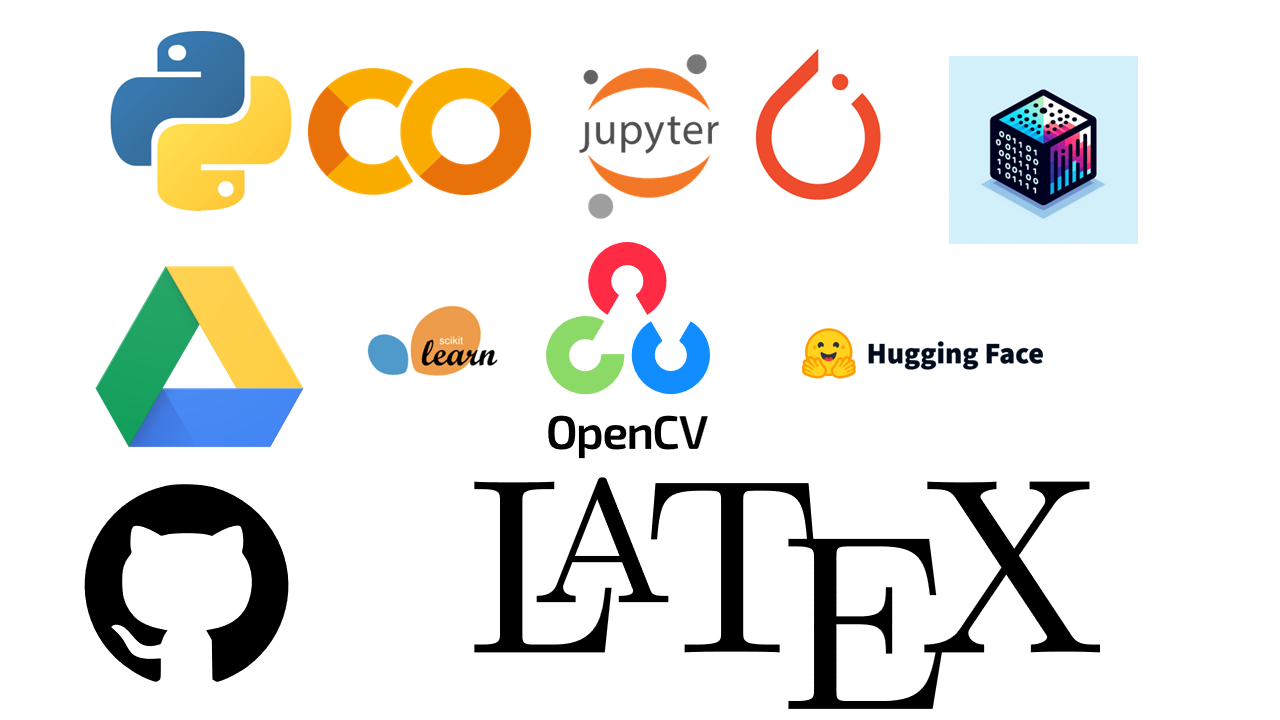
\includegraphics[width=0.9\textwidth]{Figuras/TecnologiasUsadas.png}
    \caption{Tecnologías usadas para el desarrollo del TFM}
    \label{fig:tecnologiasUsadas}
\end{figure}

Como se puede observar en la \autoref{fig:tecnologiasUsadas}, las principales herramientas utilizadas han sido las siguientes: 
\begin{itemize}
    \item \textbf{\textit{Python}}: Lenguaje de programación principal de todo el proyecto, elegido por su flexibilidad, su inmenso ecosistema de librerías científicas y su estandarización absoluta en la comunidad de \textit{Data Science} y el aprendizaje automático.
    \item \textbf{\textit{Google Colab Pro} y \textit{Jupyter Notebook}}: Como entorno de desarrollo interactivo se han utilizado cuadernos de \textit{Jupyter} a través de la plataforma \textit{Google Colab}. En concreto, se ha hecho uso de recursos avanzados (aceleradores de hardware como las \textit{GPU NVIDIA L4}) para llevar a cabo el entrenamiento de modelos masivos. En total se han consumido unas 300 unidades informáticas. 
    \item \textbf{\textit{PyTorch}}: \textit{Framework} de \textit{Deep Learning} que ha servido como núcleo matemático para construir, entrenar y evaluar todos los modelos basados en \textit{Transformers} implementados en la fase empírica. 
    \item \textbf{Ecosistema \textit{Hugging Face}}: Plataforma y conjunto de bibliotecas clave en el proyecto. Se ha utilizado para importar modelos preentrenados (\textit{Mistral}, \textit{LLaMA}, \textit{Gemma}, \textit{ConvNeXt}, etc.), aplicar técnicas de \textit{PEFT} mediante inserción de matrices de bajo rango, ejecutar optimizadores supervisados como \textit{SFTTrainer}, y formatear eficientemente los conjuntos de datos.
    \item \textbf{\textit{BitsAndBytes}}: Librería fundamental de optimización de hardware que ha permitido aplicar la técnica de cuantización \textit{QLoRA}, reduciendo los pesos de los \textit{LLMs} a una precisión de 4 bits para que pudieran ser procesados en la memoria de la tarjeta gráfica disponible. 
    \item \textbf{\textit{Decord} y \textit{OpenCV} (\textit{cv2})}: Bibliotecas especializadas en el procesamiento audiovisual. Han sido fundamentales para el tratamiento de la modalidad de vídeo, permitiendo una lectura optimizada de los archivos multimedia y la extracción precisa de los fotogramas clave (\textit{frames}) requeridos por los modelos visuales. 
    \item \textbf{\textit{Scikit-Learn} y \textit{Evaluate}}: Herramientas de análisis de datos utilizadas en la fase de evaluación para computar métricas complejas de rendimiento (\textit{F1-Score}, \textit{Accuracy}, matrices de confusión) sobre los conjuntos de prueba estáticos.
    \item \textbf{\textit{Google Drive}}: Sistema de almacenamiento en la nube utilizado como repositorio de datos centralizado. Ha servido para alojar, gestionar y sincronizar todos los conjuntos de datos (\textit{datasets}), los pesos de los modelos guardados y los archivos generados durante la experimentación, permitiendo una integración y un acceso directo desde los entornos de \textit{Google Colab}.
    \item \textbf{\textit{GitHub}}: Plataforma de desarrollo colaborativo y control de versiones. Se ha empleado para estructurar de forma metódica y segura el proyecto mediante repositorios independientes: uno destinado a la centralización del código fuente y los cuadernos de experimentación \footnote{\url{https://github.com/visumania/DeepSexist}}, y otro para el control de versiones de la presente memoria \footnote{\url{https://github.com/visumania/MemoriaTFM}}. 
    \item \textbf{\textit{LaTeX}}: Sistema de composición de textos utilizado para la redacción, estructuración y maquetación de esta memoria. Su elección garantiza un formato académico riguroso, así como una gestión impecable de las referencias bibliográficas y la representación de fórmulas matemáticas. 
\end{itemize}

A modo de conclusión, en este capítulo se han establecido los fundamentos teóricos necesarios para comprender los enfoques tecnológicos implementados a lo largo del proyecto. Esta base conceptual resulta indispensable para justificar las decisiones técnicas, algorítmicas y metodológicas que se abordarán en detalle en el próximo capítulo. 